% Содержимое отчета по курсу Анализ алгоритмов

\aaunnumberedsection{ВВЕДЕНИЕ}{sec:intro}

В данной лабораторной работе рассматриваются параллельные вычисления на основе нативных потоков.

Цель работы -- получение навыка организации параллельных вычислений на основе нативных потоков. 

Задачи работы: 
\begin{itemize}
    \item анализ предметной области;
    \item разработка алгоритма выгрузки данных со страниц сайта eda.ru~\cite{eda};
    \item создание ПО, реализующего разработанный алгоритм;
    \item исследование зависимости производительности разработанного ПО от количества дополнительных потоков.
\end{itemize}

\aasection{Входные и выходные данные}{sec:input-output}

Входными данными являются адрес главной страницы ресурса (eda.ru~\cite{eda}, адрес главной страницы не может быть изменён пользователем), максимальное число скачиваемых страниц, количество дополнительных потоков (при получении 0 дополнительные потоки не создаются). Выходными данными является директория output с файлами, содержащими файлы с выгруженными данными со страниц в формате html.

\aasection{Преобразование входных данных в выходные}{sec:algorithm}
 
Программа выгружает данные с главной страницы eda.ru~\cite{eda} в файл, после чего ищет в нём ссылки на другие страницы данного сайта. далее файл удаляется, а для найденных страниц процедура повторяется. Файлы, в которые были выгружены страницы с рецептами, не удаляются. Ссылкой на страницу с рецептом будет считаться ссылка вида eda.ru/recepty/категория/название. Процесс заканчивается либо после выгрузки достаточного количества страниц, либо после выгрузки всех страниц, если их оказалось меньше.

\aasection{Примеры работы программы}{sec:demo}

Для реализации данной лабораторной работы был выбран язык $Java$, так как он содержит все необходимые средства для реализации алгоритмов. Нативные потоки создавались при помощи класса $Thread$~\cite{thread} через явный вызов конструктора.

На рисунке~\ref{fig:console} представлен пример ввода данных для программы. На рисунке~\ref{fig:folder} представлена папка с выгруженными файлами с рецептами. 

\begin{figure}[h!]
	\centering
	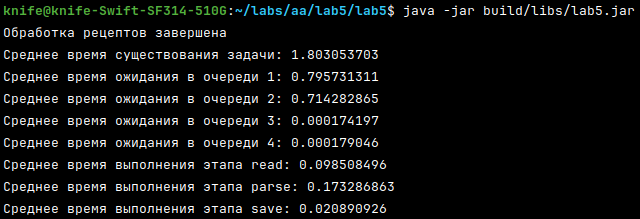
\includegraphics[width=0.9\textwidth]{console.png}
	\caption{\label{fig:console}Запуск программы}
\end{figure}

\begin{figure}[h!]
	\centering
	\includegraphics[width=0.9\textwidth]{folder.png}
	\caption{\label{fig:folder}Папка с рецептами}
\end{figure}


\aasection{Тестирование}{sec:tests}

Выполнено тестирование программы по методологии чёрного ящика. В таблице~\ref{tab:tests} представлены функциональные тесты. Первое число во вводе означает количество выгружаемых страниц, второе -- число дополнительных потоков. Все тесты пройдены успешно.

\begin{table}[h!]
	\small
	\caption{\label{tab:tests}Результаты выполнения функциональных тестов}
	\begin{center}
		\begin{tabular}{|c|c|c|c|}
			\hline
			№  & Ввод & \makecell{Ожидаемое\\количество\\страниц} & \makecell{Полученное\\количество\\страниц} \\  
			\hline
			1 & 10 0 & 10 & 10 \\
			\hline
			2 & 10 1 & 10 & 10 \\
			\hline
			3 & 10 3 & 10 & 10 \\
			\hline
			4 & 25 0 & 10 & 10 \\
			\hline
			5 & 25 1 & 10 & 10 \\
			\hline
			6 & 25 3 & 10 & 10 \\
			\hline
			7 & 100 0 & 10 & 10 \\
			\hline
			8 & 100 1 & 10 & 10 \\
			\hline
			9 & 100 3 & 10 & 10 \\
			\hline
		\end{tabular}
	\end{center}
\end{table}

\aasection{Описание исследования}{sec:study}

Было проведено исследование зависимости скорости работы программы от числа потоков в терминах числа выгруженных страниц с рецептами в минуту. Для замеров времени работы программа выгружала 1000 рецептов, после чего выводилось среднее количество выгруженных страниц в минуту. Время работы было замерено с помощью метода $System.nanoTime()$~\cite{nanotime}. Все замеры проводились на ноутбуке Acer Swift 3x, процессор 11th Gen Intel(R) Core(TM) i7-1165G7~\cite{intel}, 4 ядра. 

Измерения проводились для 0, 1, 2, 4, 8 и 16 дополнительных потоков. Результаты представлены на рисунке~\ref{fig:res}.

\clearpage

\begin{figure}[h!]
	\centering
	\includegraphics[width=0.8\textwidth]{work_graph.pdf}
	\caption{\label{fig:res} Результаты измерений числа выгруженных страниц в минуту}
\end{figure}

Наибольшая скорость работы была достигнута при совпадении числа потоков с количеством ядер в процессоре. При меньшем числе потоков скорость работы прямо пропорциональна числу потоков (при этом в случаях отсутствия дополнительных потоков и наличия 1 дополнительного потока работает приблизительно с одной и той же скоростью, так как в каждом случае только один поток выполняет вычисления), а при большем -- обратно пропорциональна, так как большее число потоков не может быть запущено, но при этом увеличиваются затраты на диспетчеризацию.

\aaunnumberedsection{ЗАКЛЮЧЕНИЕ}{sec:outro}

Цель работы достигнута. Решены все поставленные задачи: 
\begin{itemize}
    \item анализ предметной области;
    \item разработка алгоритма выгрузки данных со страниц сайта eda.ru~\cite{eda};
    \item создание ПО, реализующего разработанный алгоритм;
    \item исследование зависимости производительности разработанного ПО от количества дополнительных потоков.
\end{itemize}
